\chapter{Test cases}
\label{cap:testgen}

In this section, we will be concerned with test case creation from the functional perspective. The structure of the code will not be analyzed. Instead, the specifications with the requisites are going to be the source to derive the test cases.

\input sec-testcasedesign

\input sec-autotestcases

\section{Automatic execution of test cases}

\section{Implementation of test case generation for statecharts}
\label{implementTestGen}

In this project, we implemented the test case generation for statecharts based on the criteria described in \cite{bogdanov}. We test every transition by visiting every state and trigger events for all transitions that start in it. 

\subsection{Test case for simple statecharts}
\label{testSimpeState}

For this section, we consider only statecharts that do not contain hierarchy and concurrency. Statecharts with hierarchy and concurrency will be explained later.


We start by making sure every reachable state in the statechart is covered. In order to do so, for each state $s$ in the statechart, we construct a path $p$ from the initial state to $s$. The path $p$ in said to be the coverage path of $s$. All coverage paths generated are stored in a set called \textit{State Cover}, which is denoted by $C$. Therefore, $C$ is a set of sequence of transition labels, such that we can find an element from this set to reach any desired state starting from the initial one \cite{bogdanov}.

Since there is no hierarchy or concurrency in the statechart, the construction of $C$ is similar to covering states of an automaton. The process can be done through a depth search:

@@@@@ ADICIONAR PSEUDO-CODIGO DA COBERTURA

Now that we have the coverage for every reachable state, we need to trigger each transition on each state and create the test cases. For each transition there will be a test case, thus every transition in the diagram will be exercides at least once during testing.

Consider the transition $t = (s,l,q)$, where $s$ is the original state, $l$ is the event label that triggers $t$ and $q$ is the destinity state. Previously, we computed that $s$ has coverage path $p$ such that $p \in C$ and $p$ is a sequence of label. The test case $TC$ to $t$ would be the concatenation of the event label $l$ to the end of $p$ expecting to get to state $q$. The process is repeated to every transition in the statechart.

Consider the following example in figure \ref{fig:trocaPlano} where we model the verifications in a purchase flow of a telco ecommerce. The flow is done by a user who wishes to change their cellphone plan. They will be able to change plan if their not employees from the telco company and are not committed to a loyalty contract.

\begin{figure}[htb]
\centering
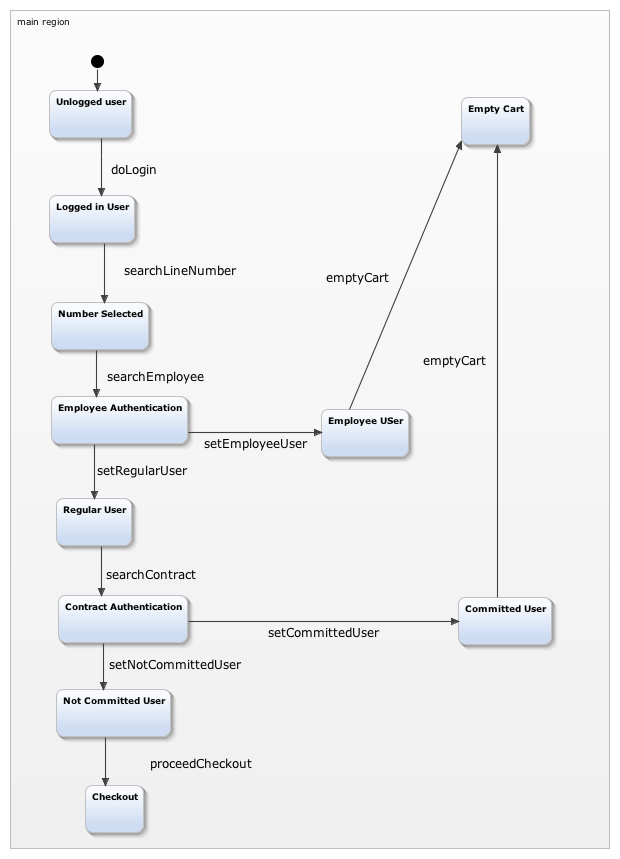
\includegraphics[width=10cm]{figuras/trocaPlano}
\caption{\label{fig:trocaPlano} A plan change flow statechart in a telco ecommerce}
\end{figure}

Hierarchy and orthogonality are not found in statechart \ref{fig:trocaPlano}. Hence, we can apply the the technique just presented.

The construction of the \textit{State Cover} set, or $C$, goes as follows:

We start at the inital state \textit{Unlogged User}. Since it is the initial state, its coverage path is the emtpy string, denoted by $e$.

Next, we recursively visit the states that can be reached from \textit{Unlogged User}. In our example, we get to state \textit{Logged in User}. In order to get to this state, it was necessary to go through transition $doLogin$. Therefore, the coverage path for \textit{Logged in User} is \textit{e doLogin}. Note that we concatenate the coverage path of the previous state to the transition taken.

When construction of $C$ is done, we have the following covage paths:

\begin{center}
\begin{tabular}{| l | p{10cm}|}

\hline

State & Coverage path \\ \hline

Unlogged user & e \\ \hline

Logged in User & e doLogin\\ \hline 

Number Selected & e doLogin searchLineNumber\\ \hline

Employee Authentication & e doLogin searchLineNumber searchEmployee\\ \hline

Employee User & e doLogin searchLineNumber searchEmployee setEmployeeUser \\ \hline

Empty Cart & e doLogin searchLineNumber searchEmployee setEmployeeUser emptyCart \\ \hline

Regular User & doLogin searchLineNumber searchEmployee setRegularUser \\ \hline

Contract Authentication & doLogin searchLineNumber searchEmployee setRegularUser searchContract \\ \hline

Committed User & doLogin searchLineNumber searchEmployee setRegularUser searchContract setCommittedUser \\ \hline

Not Committed User & doLogin searchLineNumber searchEmployee setRegularUser searchContract setNotCommittedUser \\ \hline

Checkout & doLogin searchLineNumber searchEmployee setRegularUser searchContract setNotCommittedUser proceedCheckout\\
\hline
\end{tabular}
\end{center}

Then, we have to create a test case for every transition leaving each state. Let's take state \textit{Employee Authentication} for example. It has two leaving transitions: $setEmployeeUser$ and $setRegularUser$. To guarantee they are exercided at least once during testing and that they go to their appropriate destinity states, we need the following test cases:

\begin{itemize}

\item Test case for \textit{\textbf{setEmployeeUser}}

Path: \textit{e doLogin searchLineNumber searchEmployee setEmployeeUser}

Expected state: \textit{Employee User}

\item Test case for \textit{\textbf{setRegularUser}}

Path: \textit{e doLogin searchLineNumber searchEmployee setRegularUser}

Expected state: \textit{Regular User}
\end{itemize}

Note that the path to test is the coverage page of the origin state concatenated with the label of the tested transition. The analogous is done for all other transitions in the model.

\subsection{Test case for complex statecharts: hierarchy}


In this section, the test cases generated will be obtained from statecharts that have hierarchy: a state may contain many substates and so on. We do not limit the level of nested hierarchy for the automatic generation. Consider states $A$ and $B$, such that $A$ contains $B$. We will $a$ the superstate of $b$ and $b$ the substate of $a$.

One way to deal with hierarchy is to eliminate it from the model by flattening the statechart as shown in \ref{flattening}. The statechart would become an automaton and the thecniques for simple statecharts explained in the previous section could be used to generate test cases. But, the approach taken in this project, as in \cite{bogdanov}, was to keep the structure of the statechart and create the test cases incrementally.

Similarly to the previous simpler case, for statecharts with hierarchy we still need to cover all states by constructing the set $C$ and then test all transitions in the model. The construction of $C$, however, needs to take into consideration substates to cover them as well. It is important to note that we considered only statecharts that do not have transitions between different hierarchy levels. 

When we get to a state, we should check if it contains substates. If it does, we can compute substates' coverage paths going deeper in the hierarchy level. Later, we concatenate the coverage path of the superstate to the begining of each coverage path of the substates. Then, the coverage path of the super state should be removed from $C$ and the paths to the substates will be kept in $C$ instead. Besides, consider the case in which the coverage path $p$ of a certain state $s$ passes through a superstate $q$. We need to mark in $p$ that it passed by $q$ and that the coverage paths of $q$'s substates should be used when creating test cases for transitions leaving $s$.

The algorithm to construct $C$ needs some changes then:

@@@@@ALGORITMO PARA NOVA CONSTRUCAO DO C 

After the set $C$ is complete, we need to in fact create the test cases based on every transition that leaves each state. In states that do not have substates andd whose coverage did not pass by a superstate, the process is the one presented in the previuos section. In case, the state's coverage path went through a superstate,  If a state contains substates, however, we must transfer the origin of every transition that leaves it to each one of its substates. Consider the case that a state $s$ has a transition $t = (s,l,q)$ and contains substates $s_1, s_2$ and $s_3$. When creating the test case to $t$, we will actually consider three new transitions: $t_1 = (s_1,l,q), t_2 = (s_2,l,q)$ and $t_3 = (s_3,l,q)$. 

@@@@@ALGORTIMO PARA EXPANSAO DOS COVERAGE PATHS

@@@@@ALGORITMO PARA TRANSFERIR TRANSICOES DE PAI PARA FILHO

Let's take as an example the statechart in figure \ref{fig:webEDI}. It models an application that receives order files in a specific format and converts them into an well formatted xml. Each order file contains several lines, and each line contains a product and its quantity. The application also has an integration layer, that will receive the xml file and then send it to the management system.

\begin{figure}[htb]
\centering
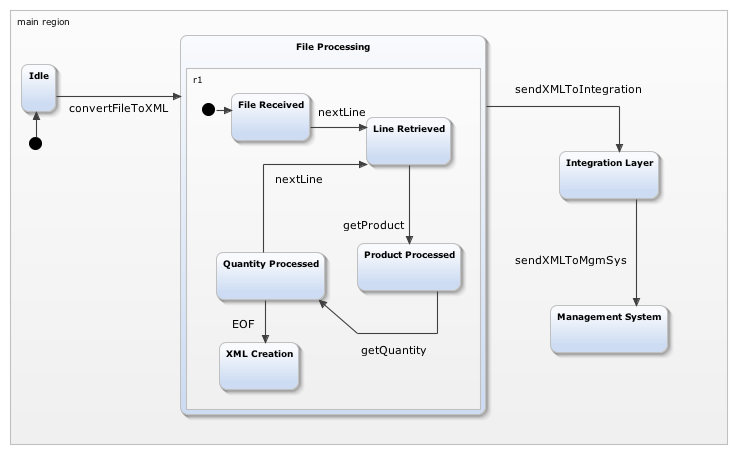
\includegraphics[width=15cm]{figuras/webEDI}
\caption{\label{fig:webEDI} Statechart for order file processing and transference}
\end{figure}

In figure \ref{fig:webEDI}, to contruct the coverage path to \textit{Idle} we do not need to worry about hierarchy, so approach described in the prior section (\ref{testSimpeState}) is enough.

\begin{center}
\begin{tabular}{| l | l|}

\hline

State & Coverage path \\ \hline

Idle & e \\

\hline
\end{tabular}
\end{center}

When creating the coverage path for state \textit{File processing}, we notice that it actually is superstate. So, instead, we go deeper in the hierarchy level to obtain the coverage paths of substates \textit{File received, Line retrieved, Product processed, Quantity processed} and \textit{XML creation}. We should add the following paths to set $C$:

\begin{center}
\begin{tabular}{| l | l|}

\hline

State & Coverage path \\ \hline

File received & e convertFileToXML e \\ \hline

Line retrieved & e convertFileToXML e nextLine\\ \hline

Product processed & e convertFileToXML e nextLine getProduct\\ \hline

Quantity processed & e convertFileToXML e nextLine getProduct getQuantity\\ \hline

XML creation & e convertFileToXML e nextLine getProduct getQuantity EOF\\ 

\hline
\end{tabular}
\end{center}

Notice that the coverage path for the superstate \textit{File processing} is removed from $C$, because we are considering its substates. Therefore, the testcases that would be created based on the superstate will be created based on the substates.

We still need to cover states \textit{Integration layer} and \textit{Management system}. Observe that to cover these states, we need to pass by \textit{File processing}, a superstate. Therefore, in their coverage path, we need to use a specific notation to guide the later expansion with the substates coverage paths. We will use the notation $\Delta_{File\ processing}$ to indicate that, when creating the test cases, we need to expand the path considering the coverage of \textit{File processing}'s substates. Thus, the coverage paths for \textit{Integration layer} and \textit{Management system} are as follows:

\begin{center}
\begin{tabular}{| l | p{10cm}|}

\hline

State & Coverage path \\ \hline

Integration layer & e convertFileToXML $\Delta_{File\ processing}$ sendXMLToIntegration \\ \hline

Management system & e convertFileToXML $\Delta_{File\ processing}$ sendXMLToIntegration sendXMLToMgmSys\\

\hline
\end{tabular}
\end{center}

At this point, that we have the complete set $C$, we start to in fact create the test cases. As an example, we will examine transitions \textit{getProduct, sendXMLToIntegration} and \textit{sendXMLToMgmSys} more closely.

For \textit{getProduct}, a transition leaving a substate, the process will be the same one presented in the previous section (\ref{testSimpeState}). Hence, we have the following test case:

\begin{itemize}

\item Test case for \textit{\textbf{getProduct}}

Path: \textit{e convertFileToXML e nextLine getProduct}

Expected state: \textit{Product processed}

\end{itemize}

In the case of \textit{sendXMLToIntegration}, a transition that leaves a superstate, we need to use the information regarding the substates to create the test cases. For each substate's coverage path $p$, there will be a test case for \textit{sendXMLToIntegration} making usage of $p$. We should append $sendXMLToIntegration$ to each $p$ in order to obtain the test paths:

\begin{itemize}

\item Test case \#1 for \textit{\textbf{sendXMLToIntegration}}

Path: \textit{e convertFileToXML e sendXMLToIntegration}

Expected state: \textit{Integration layer}

\item Test case \#2 for \textit{\textbf{sendXMLToIntegration}}

Path: \textit{e convertFileToXML e  nextLine sendXMLToIntegration}

Expected state: \textit{Integration layer}


\item Test case \#3 for \textit{\textbf{sendXMLToIntegration}}

Path: \textit{e convertFileToXML e  nextLine  getProduct sendXMLToIntegration}

Expected state: \textit{Integration layer}

\item Test case \#4 for \textit{\textbf{sendXMLToIntegration}}

Path: \textit{e convertFileToXML e  nextLine  getProduct  getQuantity sendXMLToIntegration}

Expected state: \textit{Integration layer}

\item Test case \#5 for \textit{\textbf{sendXMLToIntegration}}

Path: \textit{e convertFileToXML e  nextLine  getProduct  getQuantity EOF sendXMLToIntegration}

Expected state: \textit{Integration layer}

\end{itemize}

As for transition \textit{sendXMLToMgmSys}, the expansion of \textit{Integration layer}'s coverage path is pending. Similarly to what we did for transition \textit{sendXMLToIntegration}, we also need to consider the paths of \textit{File processing}'s substates. Therefore, the test cases for \textit{sendXMLToMgmSys} are:

\begin{itemize}

\item Test case \#1 for \textit{\textbf{sendXMLToMgmSys}}

Path: \textit{e convertFileToXML e sendXMLToIntegration sendXMLToMgmSys}

Expected state: \textit{Integration layer}

\item Test case \#2 for \textit{\textbf{sendXMLToMgmSys}}

Path: \textit{e convertFileToXML e  nextLine sendXMLToIntegration sendXMLToMgmSys sendXMLToMgmSys}

Expected state: \textit{Integration layer}


\item Test case \#3 for \textit{\textbf{sendXMLToMgmSys}}

Path: \textit{e convertFileToXML e  nextLine  getProduct sendXMLToIntegration sendXMLToMgmSys}

Expected state: \textit{Integration layer}

\item Test case \#4 for \textit{\textbf{sendXMLToMgmSys}}

Path: \textit{e convertFileToXML e  nextLine  getProduct  getQuantity sendXMLToIntegration sendXMLToMgmSys}

Expected state: \textit{Integration layer}

\item Test case \#5 for \textit{\textbf{sendXMLToMgmSys}}

Path: \textit{e convertFileToXML e  nextLine  getProduct  getQuantity EOF sendXMLToIntegration sendXMLToMgmSys}

Expected state: \textit{Integration layer}

\end{itemize}

Notice that, in each case, $\Delta_{File\ processing}$ in \textit{Integration layer}'s coverage was replaced by a substate's coverage path.

\subsection{Test case for complex statecharts: orthogonality}

Now we shall consider statecharts that possess orthogonality, in other words, states in concurrent regions.

One fisrt method to generate test cases dealing with orthogonality is to eliminate it by flattening the statechart as explained in \ref{flattening}. The elimation of orthogonality would be done with the cartesian product of all states and transitions causing an explosion in the number of result states and transitions \cite{bogdanov}.

There are some possible refinements to stablish in order to generate fewer test cases and stil get all states covered and all transitions tested. The one used for this project was the following:

\begin{itemize}

\item \textbf{Strong concurrency}

This refinement allows us to test concurrent components separately. Transitions from each concurrent region are triggered one-by-one in different steps.
The \textit{State Cover} set $C$ for this refinement is smaller than in the weak concurrency or in the state multiplication.
\end{itemize}

We first compute the covage paths for each concurrent region separately. Then, similarly to the case with hierarchy, we combine these paths with the coverage path of the state that contains the concurrent regions. After obtaining the coverage path for all states, set $C$ is complete. Find the algorithm below:

@@@@@ADICIONAR PSEUDO-CODIGO

Next, we again need to generate the test cases for each transition of the model. This process is the same as the one described in the case with hierarcy since concurrent states are inside a super state. Find example below:

@@@@@ADICIONAR EXEMPLO

